\section{1174039- Liyana Majdah Rahma}
    \subsection{Teori}
    \begin{enumerate}
        \item jelaskan kenapa file suara harus dilakukan MFCC dilengkapi dengan ilustrasi atau gambar.
        \subitem MFCC (Mel Frequency Cepstrum Coefficients) merupakan proses ekstraksi ciri dari sinyal wicara. Proses MFCC akan mengkonversikan sinyal suara menjadi beberapa vektor yang berguna untuk proses pengenalan. MFCC merupakan salah satu metode yang digunakan dalam bidang speech teknologi seperti speaaker recognition serta speech recognition. Selain itu juga spekearnya mampu Mampu untuk menangkap karakteristik suara yang sangat penting bagi pengenalan suara, serta dapat menangkap informasi-informasi penting yang terkandung dalam signal suara. Dapat dilihat seperti gambar dibawah ini
        \begin{figure}[H]
            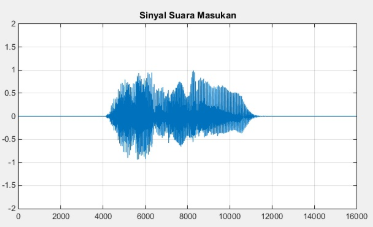
\includegraphics[width=4cm]{figures/1174039/chapter6/teori1.png}
            \centering
            \caption{Ilustrasi gambar metode MFCC}
        \end{figure}
        
        \item Jelaskan konsep dasar neural network. dilengkapo dengan ilustrasi gambar.
        \subitem Konsep dasar neural network sendiri di mulai dari ide dasar neural network dari otak manusia, dimana otak terdiri dari 1011 neuron. sehingga konsep dasar ini membangun neural network buatan yang disebut (Artificial Neural Network). Dapat dilihat seperti gambar dibawah ini
        \begin{figure}[H]
            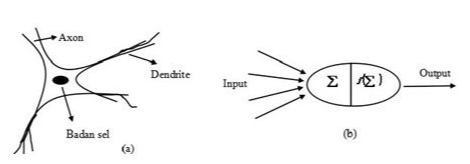
\includegraphics[width=4cm]{figures/1174039/chapter6/teori2.png}
            \centering
            \caption{Ilustrasi Konsep dasar neural network}
        \end{figure}
        
        \item Jelaskan konsep pembobotan  dalam neural network. dilengkapidengan ilustrasi gambar.
        \subitem konsep pembobotan dalam neural network sendiri menggunakan algoritma backpropagation untuk memperkecil tingkat eror dengan menyesuaikan nilai bobot berdasarkan perbedaan output serta target yang dicapai. Dapat dilihat seperti gambar dibawah ini
        \begin{figure}[H]
            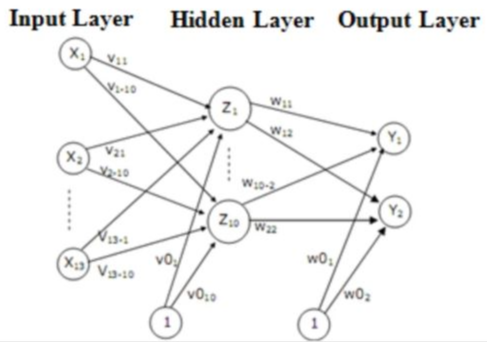
\includegraphics[width=4cm]{figures/1174039/chapter6/teori3.png}
            \centering
            \caption{Ilustrasi Konsep pembobotan pada neural network}
        \end{figure}
        
        \item jelaskan konsep aktifitas dalam neural network. dilengkapi dengan ilustrasi gambar.
        \subitem fungsi aktivasi sendiri menggunakan nilai threshold untuk membatasi nilai keluaran agar selalu dalam batas nilai yang ditetapkan. Dapat dilihat seperti gambar dibawah ini
        \begin{figure}[H]
            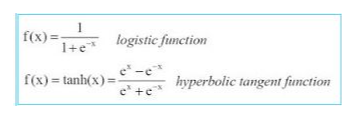
\includegraphics[width=4cm]{figures/1174039/chapter6/teori4.png}
            \centering
            \caption{Gambar yang dibaca hasil plotnya}
        \end{figure}
        
        \item Jelaskan cara membaca hasil plot dari MFCC dilengkapi dengan ilustrasi gambar. 
        \subitem Mcara membaca plot hasil mfcc dapat dilakukan dengan cara suara pengguna dijadikan file dalam bentuk *.wav yang digunakan sebagai inputan kemudian direpresentasikan menjadi sinyal suara dalam bentuk matriks dengan perintah auudiread di Matlab R2017a.Dapat dilihat seperti gambar dibawah ini
        \begin{figure}[H]
            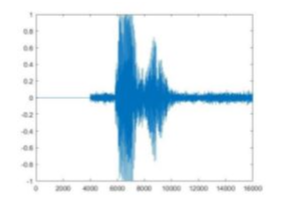
\includegraphics[width=4cm]{figures/1174039/chapter6/teori5.png}
            \centering
            \caption{Ilustrasi Cara Membaca Hasil Plot}
        \end{figure}
        
        \item Jelaskan apa itu one-hot encoding, dilengkapi dengan ilustrasi kode atau gambar.
        \subitem One Hot Encoding mengkategorikan variabel yang mengandung nilai label dan bukan nilai numerik.Dapat dilihat seperti gambar dibawah ini
        \begin{figure}[H]
            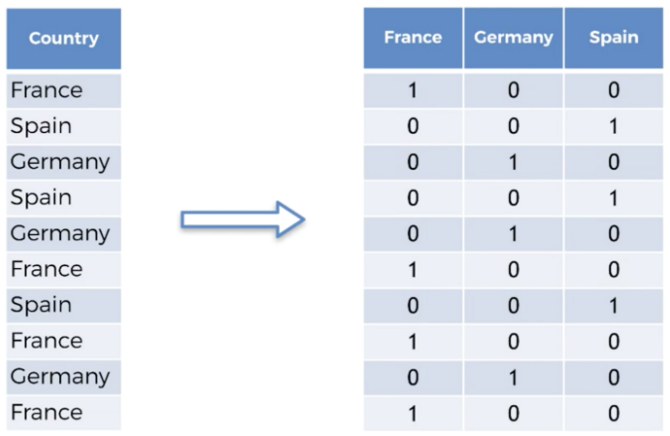
\includegraphics[width=4cm]{figures/1174039/chapter6/teori6.png}
            \centering
            \caption{Ilustrasi Konsep one-hot encoding}
        \end{figure}

        \item jelaskan apa itu fungsi np.unique dan to.categorical, dilengkapi dengan ilustrasi kode atau gambar.
        \subitem Kegunaan np array untuk keperluan analisis data, seperti operasi vektor dan matriks.Dapat dilihat seperti gambar dibawah ini
        \begin{figure}[H]
            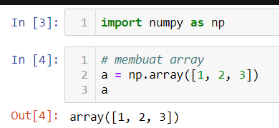
\includegraphics[width=4cm]{figures/1174039/chapter6/teori7.png}
            \centering
            \caption{Ilustrasi np.unique}
        \end{figure}

        \item Jelaskan apa fungsi dari squential dalam kode program, dilengkapi dengan ilustrasi kode atau gambar.
        \subitem Metode Sequential merupakan proses membandingkan setiap elemen larik satu per satu secara beruntun, mulai dari elemen pertama, sampai dengan elemen terakhir atau elemen yang dicari sudah ditemukan.Dapat dilihat seperti gambar dibawah ini
        \begin{figure}[H]
            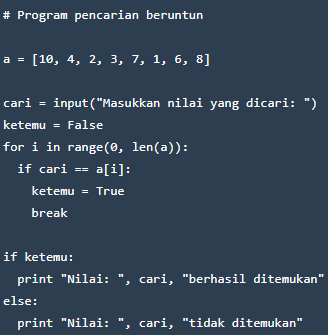
\includegraphics[width=4cm]{figures/1174039/chapter6/teori8.png}
            \centering
            \caption{Ilustrasi squential encoding}
        \end{figure}
    \end{enumerate}
    \subsection{Praktek}
        \begin{enumerate}
        \item Jelaskan isi dari data GTZAN Genre Collection dan data dari freesound. Buat kode program program untuk meload data tersebut untuk digunakan pada MFCC. Jelaskan arti dari perbaris kode yang dibuat (harus beda dengan teman satukelas).

        \item berikut adalah hasil dari Isi data yang merupakan datasets lagu atau suara yang terdiri dari 10 gendre yang di simpan kedalam 10 folder yaitu folder blues, classical, country, disco, hiphop, jazz, metal, pop, reggae, dan rock ke sepuluh folder tersebut masing-masing  berisi 100 data suara sedangkan data freesound merupakan contoh data suara yang akan di gunakan untuk menguji hasil pengolahan data tersebut dengan menggunakan metode mfcc.ilustrasi dapat dilihat pada gambar
        \begin{figure}[H]
            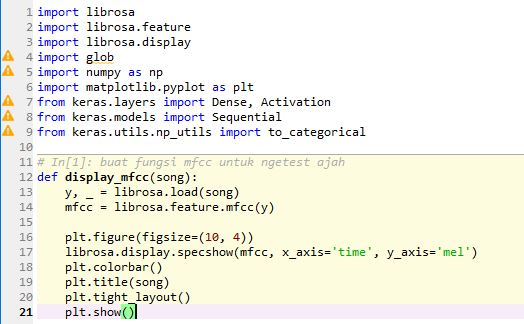
\includegraphics[width=4cm]{figures/1174039/chapter6/1.jpg}
            \centering
            \caption{Data GTZAN}
        \end{figure}
        
        \item Pada code tersebut digunakan untuk mendisplay tampilan gelombang suara yang menggunakan metode mfcc.dapat dilihat pada gambar
        \begin{figure}[H]
            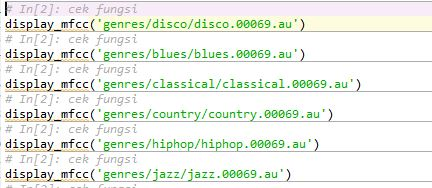
\includegraphics[width=4cm]{figures/1174039/chapter6/2.jpg}
            \centering
            \caption{hasil olah data dengan mendisplay}
        \end{figure}
        
        \item pada baris ke tiga nama extract features digunakan pada fungsi lain yang akan dibuat menjadi variabel y dengan metode librosa kemudian variabel tersebut disii dengan np.max daan variabel terakhir dibuat array dari data 250000 data pertama.dapat dilihat pada gambar
        \begin{figure}[H]
            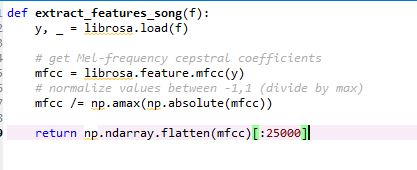
\includegraphics[width=4cm]{figures/1174039/chapter6/3.jpg}
            \centering
            \caption{hasil olah data extract features}
        \end{figure}
        
        \item  Pada baris ke tiga sebagai pendefinisian fungsi generate features dan label setelah itu buat variabel baru dengan array, kemudian isian label untuk gendre dengan cara membuat variabel genres, setiap datanya isi  dan in setelah itu akan di buat encoding untuk data tiap tiap label contoh untuk blues 1000000000 dan untuk clasical 0100000000.hasil dari pemrosesannya dapat dilihat pada gambar
        \begin{figure}[H]
            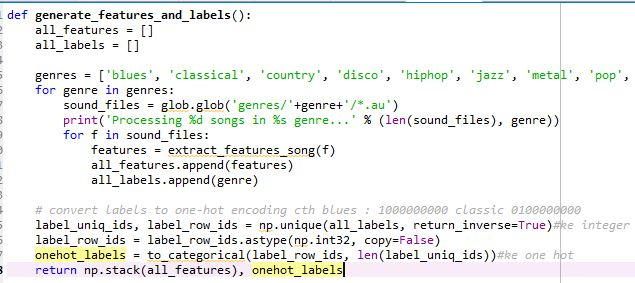
\includegraphics[width=4cm]{figures/1174039/chapter6/4.jpg}
            \centering
            \caption{hasil olah data generate features label}
        \end{figure}

        
        \item  hal ini menjadi lama dikarenakan mesin membaca satupersatu file yang ada pada folder dan dalam foldertersebut terdapat 100 file sehingga wajar menjadi lama ditambah lagi mengolah data yang tadinya suara menjadi bentuk vektor.  dapat dilihat pada gambar
        \begin{figure}[H]
            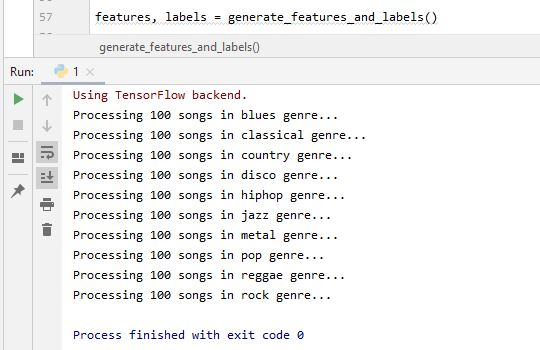
\includegraphics[width=4cm]{figures/1174039/chapter6/5.jpg}
            \centering
            \caption{hasil olah data genre}
        \end{figure}
        
        \item untuk code nya adalah sebagai berikut  yang merupakan code untuk membagi data sebanyak 80 persen untuk data training maka data musik tadi yang total jumlahnya 1000 akan di bagi dua untuk data training sebanyak 800  dan 200 untuk data testing.dapat dilihat pada gambar
        \begin{figure}[H]
            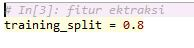
\includegraphics[width=4cm]{figures/1174039/chapter6/6.jpg}
            \centering
            \caption{hasil olah data pemisahan data training}
        \end{figure}
        
        \item  fungsi sequential digunakan untuk mengolah data inputan sesuai dengan fungsi yang ada pada fungsi sequential pada fungsi sequential kali ini menggunakan dua fungsi sequential mengkompile data dari 100 neuron atau dari 1 folder file dapat dilihat pada gambar
        \begin{figure}[H]
            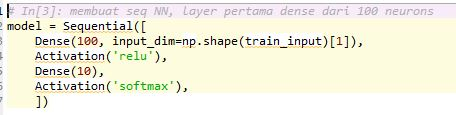
\includegraphics[width=4cm]{figures/1174039/chapter6/7.jpg}
            \centering
            \caption{hasil olah data fungsi sequential}
        \end{figure}
        
        \item  fungsi kompile yang digunakan untuk mengetahui parameter yang digunakan dari data yang telah diolah untuk caranya dapat menggunakan codingan sebagai berikut, dapat dilihat pada gambar
        \begin{figure}[H]
            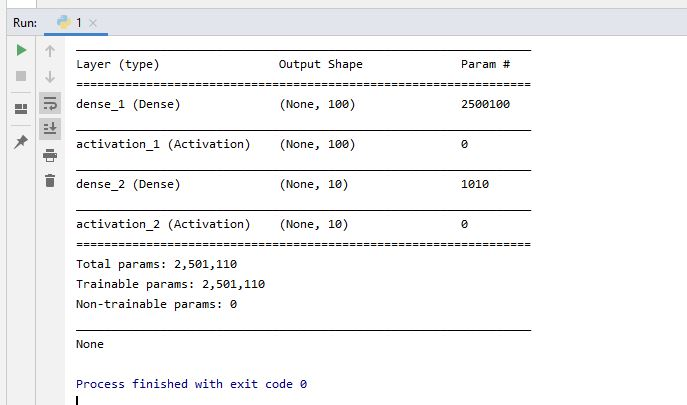
\includegraphics[width=4cm]{figures/1174039/chapter6/8.jpg}
            \centering
            \caption{hasil fungsi compile}
        \end{figure}
        
        \item  pada fungsi ini dilakukan pengolahan data dari 10 label tadi atau 10 file data sets tadi kemudian di hitung tingkat akurasi masing masing dan tingkat kegagalan atau loss data darisetiap file tersebut caranya dengan melakukan codingan berikut,dapat dilihat pada gambar
        \begin{figure}[H]
            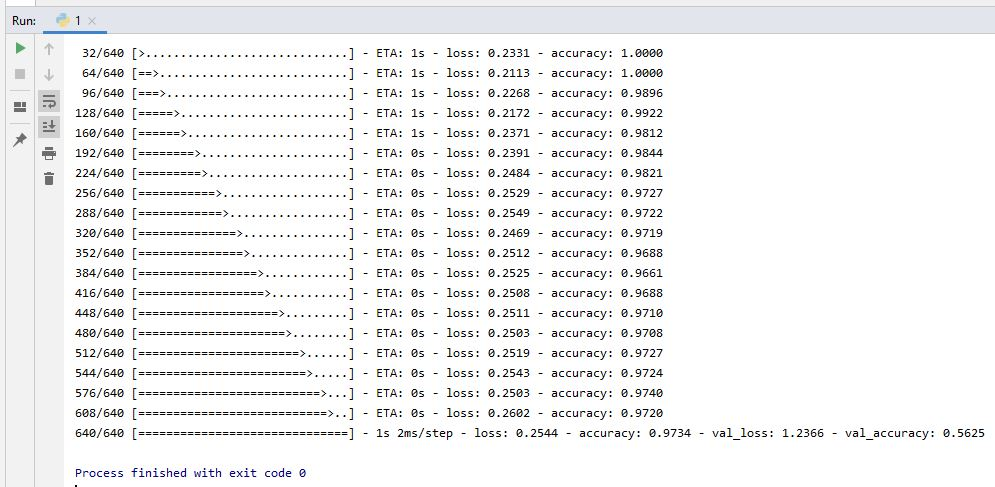
\includegraphics[width=4cm]{figures/1174039/chapter6/9.jpg}
            \centering
            \caption{hasil olah data 10 label}
        \end{figure}
        
        \item  pada fungsi ini dilakukan evaluasi terhadap datayang telah di runing sebelummnya untuk lebih jelasnya dapat di lihat codingan tersebut  pada codingan tersebut dilakukan evaluasi pada tingkat kegagalan dan akurasi kebenaran maka hasilnya munculkan hasil evaluasi dari 10 proses dari setiap gendre yaitu akurasi sebesar 51 persen dan loss data sebesar 1.4105 data.dapat dilihat pada gambar 
        \begin{figure}[H]
            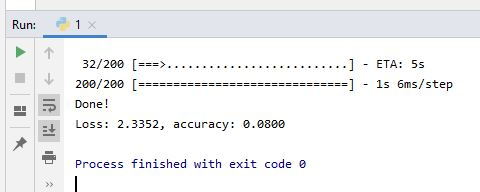
\includegraphics[width=4cm]{figures/1174039/chapter6/10.jpg}
            \centering
            \caption{hasil fungsi evaluasi}
        \end{figure}
        
        \item  fungsi predic merupakan fungsi untuk membandingkan tingkat akurasi pada setiap label yang sepuluh tadi maka data akan di sandingkan ke masing masing tingkat akurasinya, yang akurasinya paling tinggi maka itulah jawaban untuk setiap inputan yang dilakukan.dapat dilihat pada gambar
        \begin{figure}[H]
            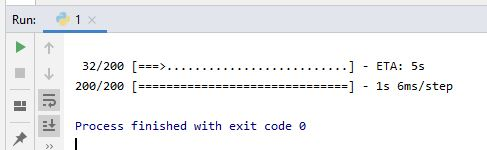
\includegraphics[width=4cm]{figures/1174039/chapter6/11.jpg}
            \centering
            \caption{hasil fungsi predict}
        \end{figure}

        \end{enumerate}